\documentclass[12pt]{beamer}
\usepackage{cmap}
\usepackage[T2A]{fontenc}
\usepackage[utf8]{inputenc}
\usepackage{ifluatex}
\usefonttheme[onlymath]{serif}
\usepackage{svg}
\usepackage{enumerate}
\usepackage{hyperref}
\usepackage{mathtools}
\setbeamertemplate{footline}[frame number]
\definecolor{beamer@darkgreen}{rgb}{0,0.6,0}
\setbeamercolor{normal text}{fg=black,bg=white}
\setbeamercolor{title}{fg=black,bg=beamer@darkgreen}
\setbeamercolor{frametitle}{fg=black,bg=beamer@darkgreen}
\setbeamercolor{background canvas}{parent=normal text}

\usepackage[english,russian]{babel}
\usepackage{graphicx}
\usepackage{listings}
\DeclareMathOperator{\sign}{sign}

\usepackage{enumerate}

\author{Катя Тузова}
\title{Машинное обучение}
\date{}


\subtitle{Лекция 13. О разном.}

\begin{document}	
\frame{\titlepage}

\begin{frame}\frametitle{MapReduce}

\end{frame}

\begin{frame}\frametitle{MapReduce}
Приложение разделяется на большое количество одинаковых элементарных заданий, выполнимых на узлах кластера и естественным образом сводимых в конечный результат. 
\end{frame}


\begin{frame}\frametitle{MapReduce}
На Map-шаге происходит предварительная обработка входных данных.

Для этого один из компьютеров получает входные данные задачи, разделяет их на части и передает другим компьютерам для предварительной обработки. Название данный шаг получил от одноименной функции высшего порядка.
\end{frame}

\begin{frame}\frametitle{MapReduce}

На Reduce-шаге происходит свёртка предварительно обработанных данных. 

Главный узел получает ответы от рабочих узлов и на их основе формирует результат — решение задачи, которая изначально формулировалась.

\end{frame}


\begin{frame}\frametitle{Hadoop}
\begin{enumerate}[--]
\item Hadoop Common
\item HDFS
\item YARN
\item Hadoop MapReduce
\end{enumerate}
\end{frame}

\begin{frame}\frametitle{Apache Mahout}
Первая большая библиотека, реализовавшая многие популярные алгоритмы средствами MapReduce.
\end{frame}

\begin{frame}\frametitle{Apache Mahout}
Алгоритмы:
\begin{enumerate}
\item Naive Bayes
\item Hidden Markov Model
\item Random Forest
\item Stochastic Gradient Descent
\item K-means
\end{enumerate}

\end{frame}


\begin{frame}\frametitle{Вопрос}
Какие проблемы возникли?
\end{frame}

\begin{frame}\frametitle{Spark}
Хочется итеративный задач на кластерах.

В MapReduce нет эффективных примитивов для общих данных.
\end{frame}


\begin{frame}\frametitle{Spark}
Решение:

Вместо того, чтобы писать в HDFS — храним в RAM.
\end{frame}

\begin{frame}\frametitle{Spark}
RDD (resilient distributed dataset) -- указатель на ленивую распределённую колекцию данных. Большинство операций над RDD не приводит к каким-либо вычислениям, а только создаёт очередную обёртку, обещая выполнить операции только тогда, когда они понадобятся.
\end{frame}


\begin{frame}\frametitle{Spark}
2 типа операторов:
\begin{enumerate}[--]
\item Трансформации -- ленивые операторы, создают новые RDD
\item Действия -- запускают вычисления и возвращают результат или пишут данные во внешнее хранилище
\end{enumerate}
\end{frame}

\begin{frame}\frametitle{Spark}

\begin{figure}[htbp]
  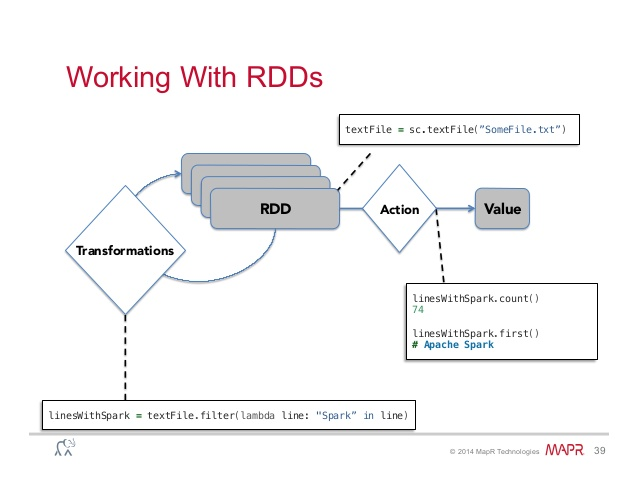
\includegraphics[height=200pt, keepaspectratio = true]{images/apache-spark-hadoop-39-638}   
\end{figure}
\end{frame}

\begin{frame}\frametitle{Spark}
Загрузка данных:

\begin{enumerate}[--]
\item Из локальной программы с помощью функции .parallelize(data)
\item Из поддерживаемых хранилищ (например, hdfs) с помощью функции .textFile(path)
\end{enumerate}

Одна из самых полезных функций -- .cache(), которая позволяет закэшировать данные в оперативной памяти. Это позволяет производить итеративные вычисления в оперативной памяти, тем самым избавившись от IO-overhead'а. 
Из коробки поддерживает интерфейсы для Scala, Java и Python.
\end{frame}

\begin{frame}\frametitle{MLLib}
%\begin{python3}
%sc = ...                                                        # создаём контекст (SparkContext)
%rdd = sc.textFile("/path/to/server_logs")     # создаём указатель на данные
%rdd.map(parse_line) \                                # разбираем строки и переводим их в удобный формат
%      .filter(contains_error) \                         # фильтруем записи без ошибок
%      .saveAsTextFile("/path/to/result")         # сохраняем результаты на диск
%\end{python3}
\end{frame}

\begin{frame}\frametitle{MLLib}
Алгоритмы:

\begin{enumerate}[--]
\item classification: logistic regression, linear support vector machine
(SVM), naive Bayes
\item regression: generalized linear regression (GLM)
\item collaborative filtering: alternating least squares (ALS)
\item clustering: k-means
\item decomposition: singular value decomposition (SVD), principal
component analysis (PCA)
\end{enumerate}
\end{frame}

\begin{frame}\frametitle{K-means}
%\begin{python3}
%# Load and parse the data
%data = sc.textFile("kmeans_data.txt")
%parsedData = data.map(lambda line:
% array([float(x) for x in line.split(' ‘)])).cache()
%# Build the model (cluster the data)
%clusters = KMeans.train(parsedData, 2, maxIterations = 10,
% runs = 1, initialization_mode = "kmeans++")
%# Evaluate clustering by computing the sum of squared errors
%def error(point):
% center = clusters.centers[clusters.predict(point)]
% return sqrt(sum([x**2 for x in (point - center)]))
%cost = parsedData.map(lambda point: error(point))
% .reduce(lambda x, y: x + y)
%print("Sum of squared error = " + str(cost))
%\end{python3}
\end{frame}

\begin{frame}\frametitle{Gradient Descent}

%val points = spark.textFile(...).map(parsePoint).cache()
%var w = Vector.random(D) // current separating plane 
%for (i <- 1 to ITERATIONS) {
%  val gradient = points.map(p =>
%   (1 / (1 + exp(-p.y*(w dot p.x))) - 1) * p.y * p.x
%  ).reduce(_ + _)
%  w -= gradient
%}
%println("Final separating plane: " + w)
\end{frame}

\begin{frame}\frametitle{Spark + Python}
\begin{enumerate}[--]
\item Python Lambdas
\item IPython Notebook
\end{enumerate}
\end{frame}

\end{document}